\section{Registro, Validación e Ingreso}

\subsection{Crear una Cuenta Nueva}
Si es tu primera vez accediendo al portal como Médico Referente, debes darte de alta para ser elegible en las listas de vinculación de los pacientes. Sigue estos pasos cuidadosamente:

\begin{enumerate}
    \item Navega a la página de inicio principal de RadiographXpress. Busca la opción \textbf{"Soy Médico Asociado"} y oprime el botón \textbf{"Crear cuenta de Médico"}.
    \item Serás redirigido a la pantalla de "Registro Profesional". Deberás completar el formulario con tus datos de contacto y acreditación médica:
    \begin{itemize}
        \item \textbf{Nombre y Apellidos:} Coloca tu nombre completo real; este será visible para los pacientes en sus listas de búsqueda.
        \item \textbf{Correo Electrónico:} Inserta una dirección de correo vigente. Este será tu usuario principal.
        \item \textbf{Cédula Profesional:} Ingresa tu número de identificación profesional otorgado por el Estado. Este campo es estrictamente evaluado.
        \item \textbf{Especialidad:} Indica tu enfoque clínico principal (ej. Traumatología, Medicina General, Pediatría, etc.).
        \item \textbf{Teléfono:} Tu número telefónico de contacto para tu consultorio.
        \item \textbf{Contraseña:} Crea una contraseña segura de al menos 8 caracteres (alfanumérica).
        \item \textbf{Confirmar Contraseña:} Vuelve a teclear la misma contraseña.
    \end{itemize}
    \item Completa el \textit{captcha} de seguridad si aparece y acepta los \textbf{Términos y Condiciones}.
    \item Haz clic en \textbf{"Crear Cuenta"}. 
\end{enumerate}

\subsection{Proceso de Verificación y Activación}
Por normativas de confidencialidad y control de calidad institucional, las cuentas de los médicos aprueban por un estado bimodal de seguridad:

\begin{enumerate}
    \item \textbf{Verificación de Correo (Automática):} El sistema enviará a tu bandeja un correo electrónico para verificar la autoría del email. Ingresa a tu correo y haz clic en el enlace adjunto.
    \begin{figure}[H]
        \centering
        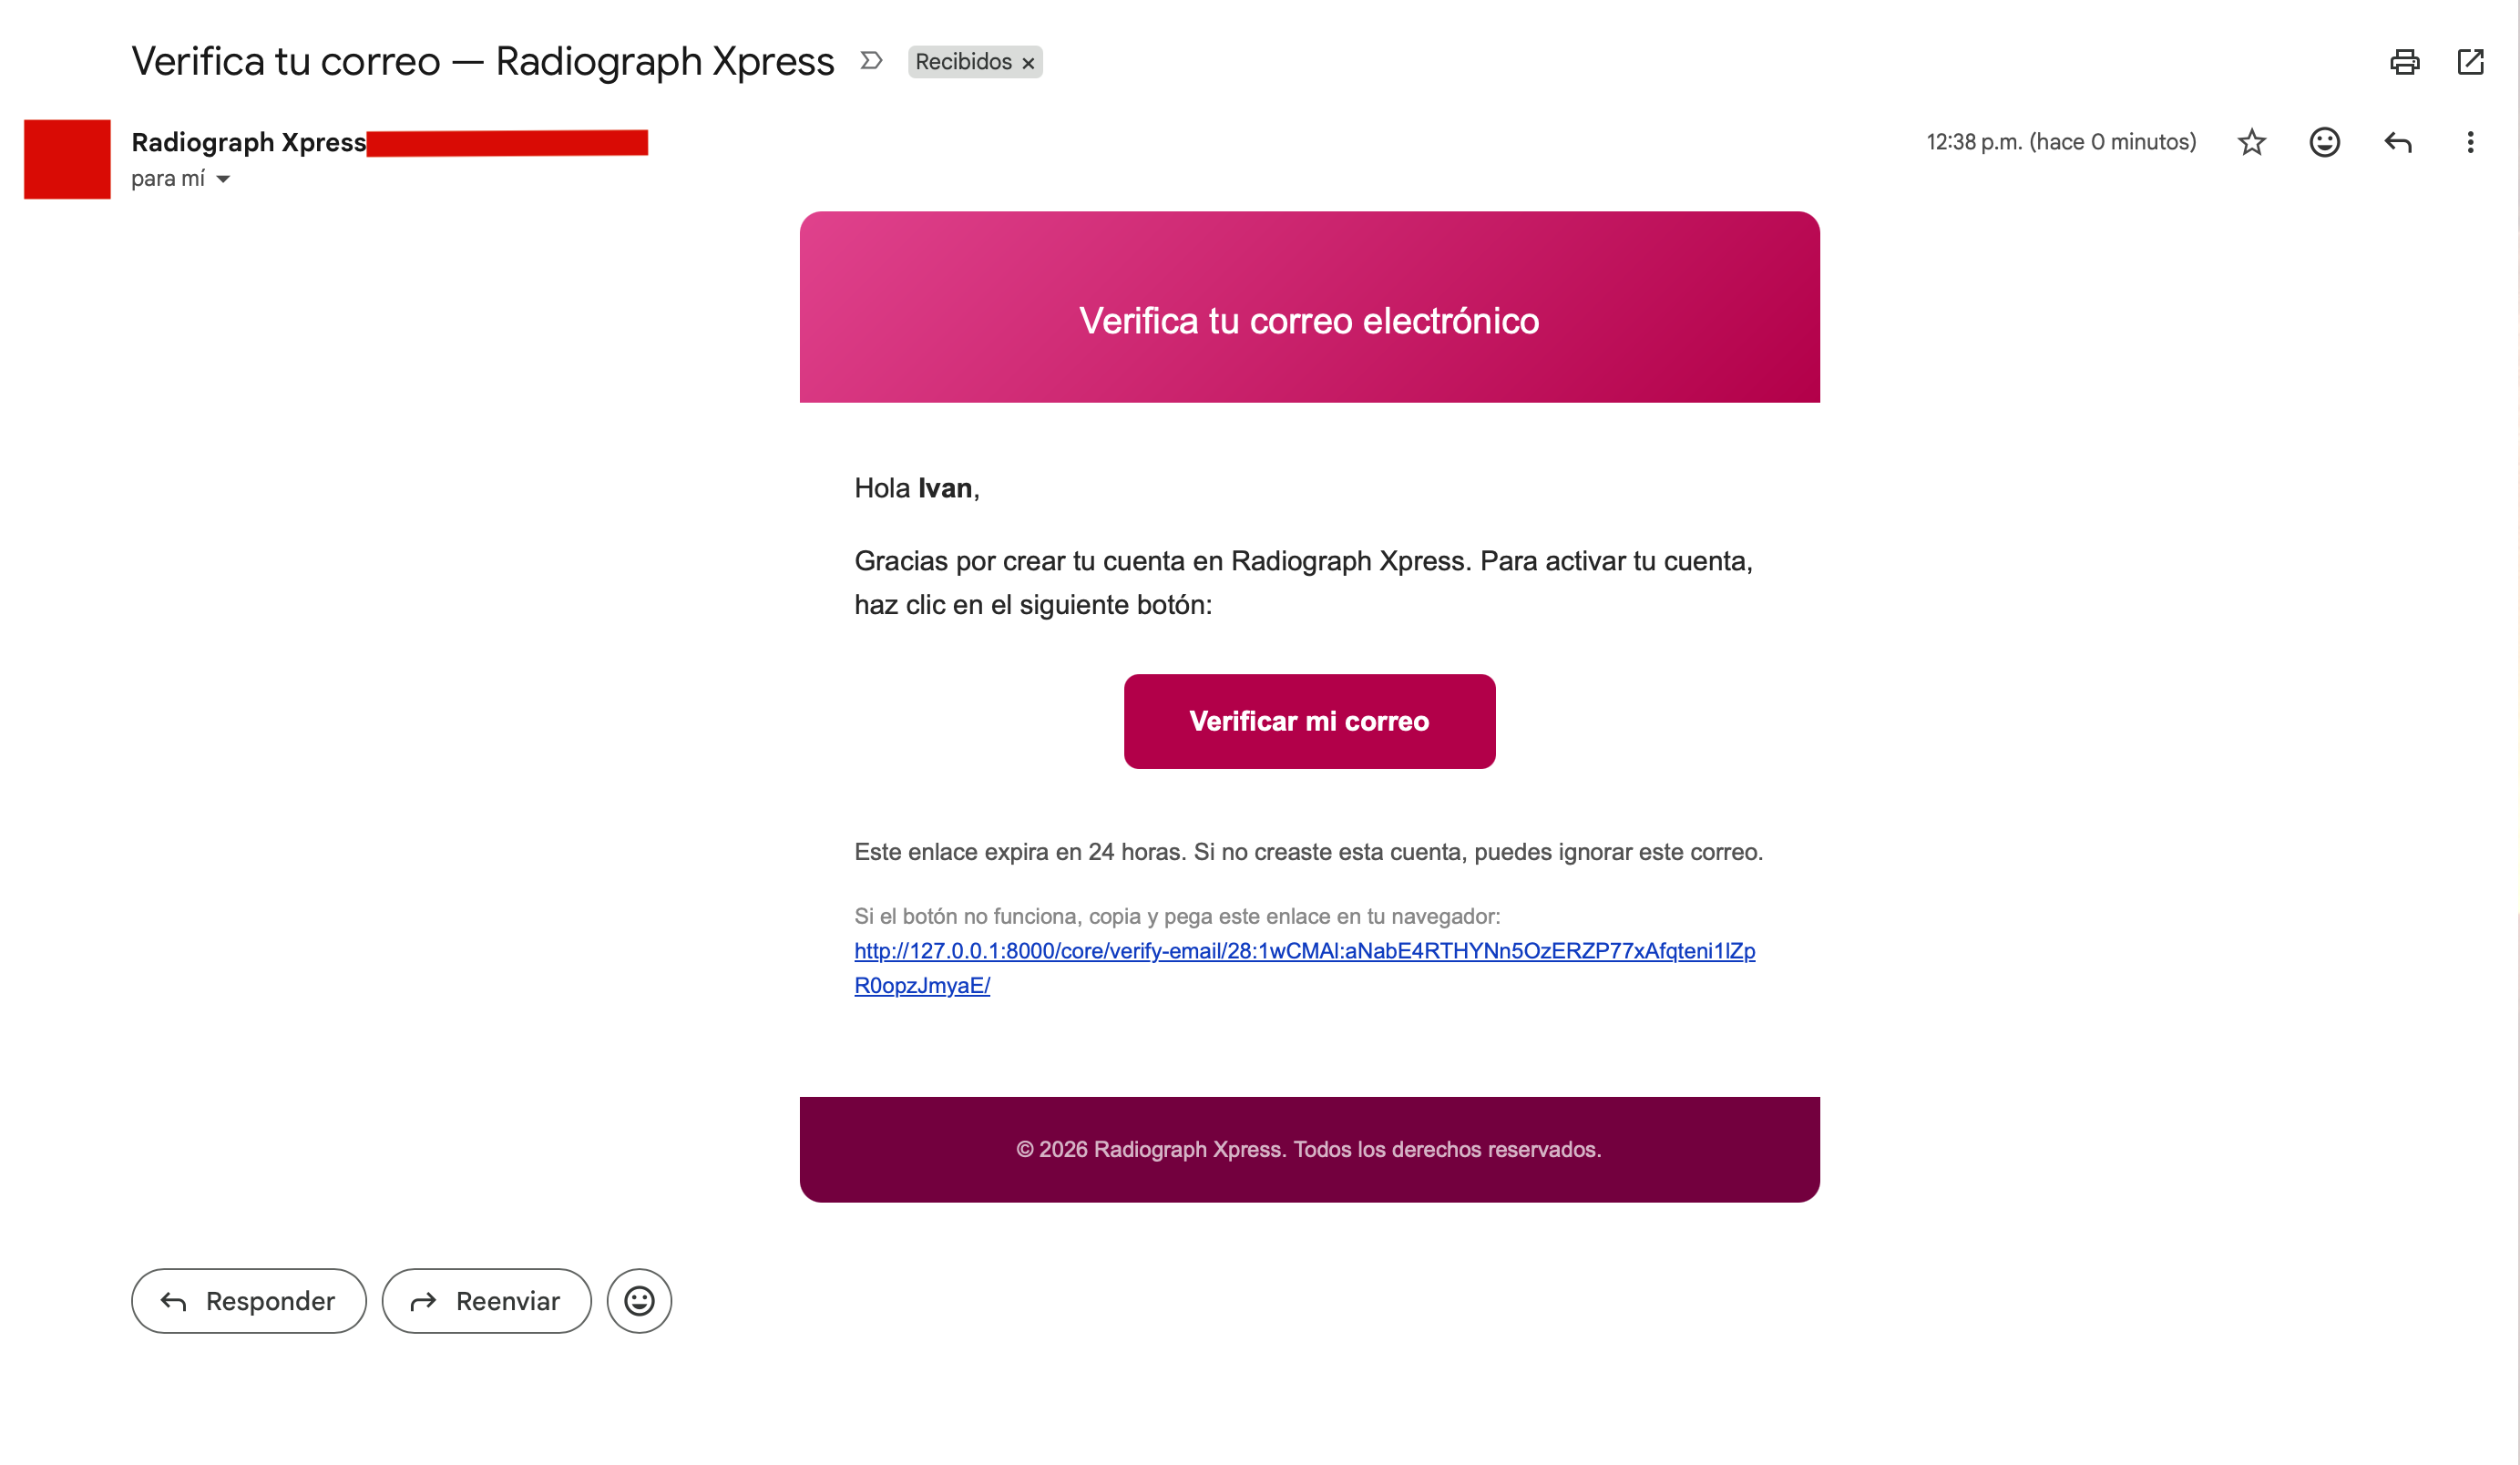
\includegraphics[width=0.5\linewidth]{screenshots/email_verification.png}
        \caption{Ejemplo de correo de verificación de cuenta.}
    \end{figure}
    \item \textbf{Validación Administrativa (Manual):} Tu cuenta continuará en "Espera de aprobación". Nuestro personal administrativo cruzará internamente tu Cédula Profesional con el Registro Público. Una vez que validen que tu estatus es vigente, autorizarán tu perfil maestro.
    \item Recibirás una notificación en cuanto el personal haya cambiado tu estado a "Aprobado", dándote acceso rotundo.
\end{enumerate}

\subsection{Iniciar Sesión}
Una vez habilitado oficialmente, ingresa al portal de forma convencional:

\begin{enumerate}
    \item Regresa a la página de inicio de sesión.
    \item En el campo \textbf{Correo Electrónico}, ingresa el correo que validaste.
    \item En el campo \textbf{Contraseña}, repite tu clave segura.
    \item Haz clic en el botón \textbf{"Iniciar Sesión"}.
    \item El sistema acreditará el acceso a tu cuenta tipo Médico Asociado y te enviará de inmediato al panel principal de tu flujo de trabajo.
    \begin{figure}[H]
        \centering
        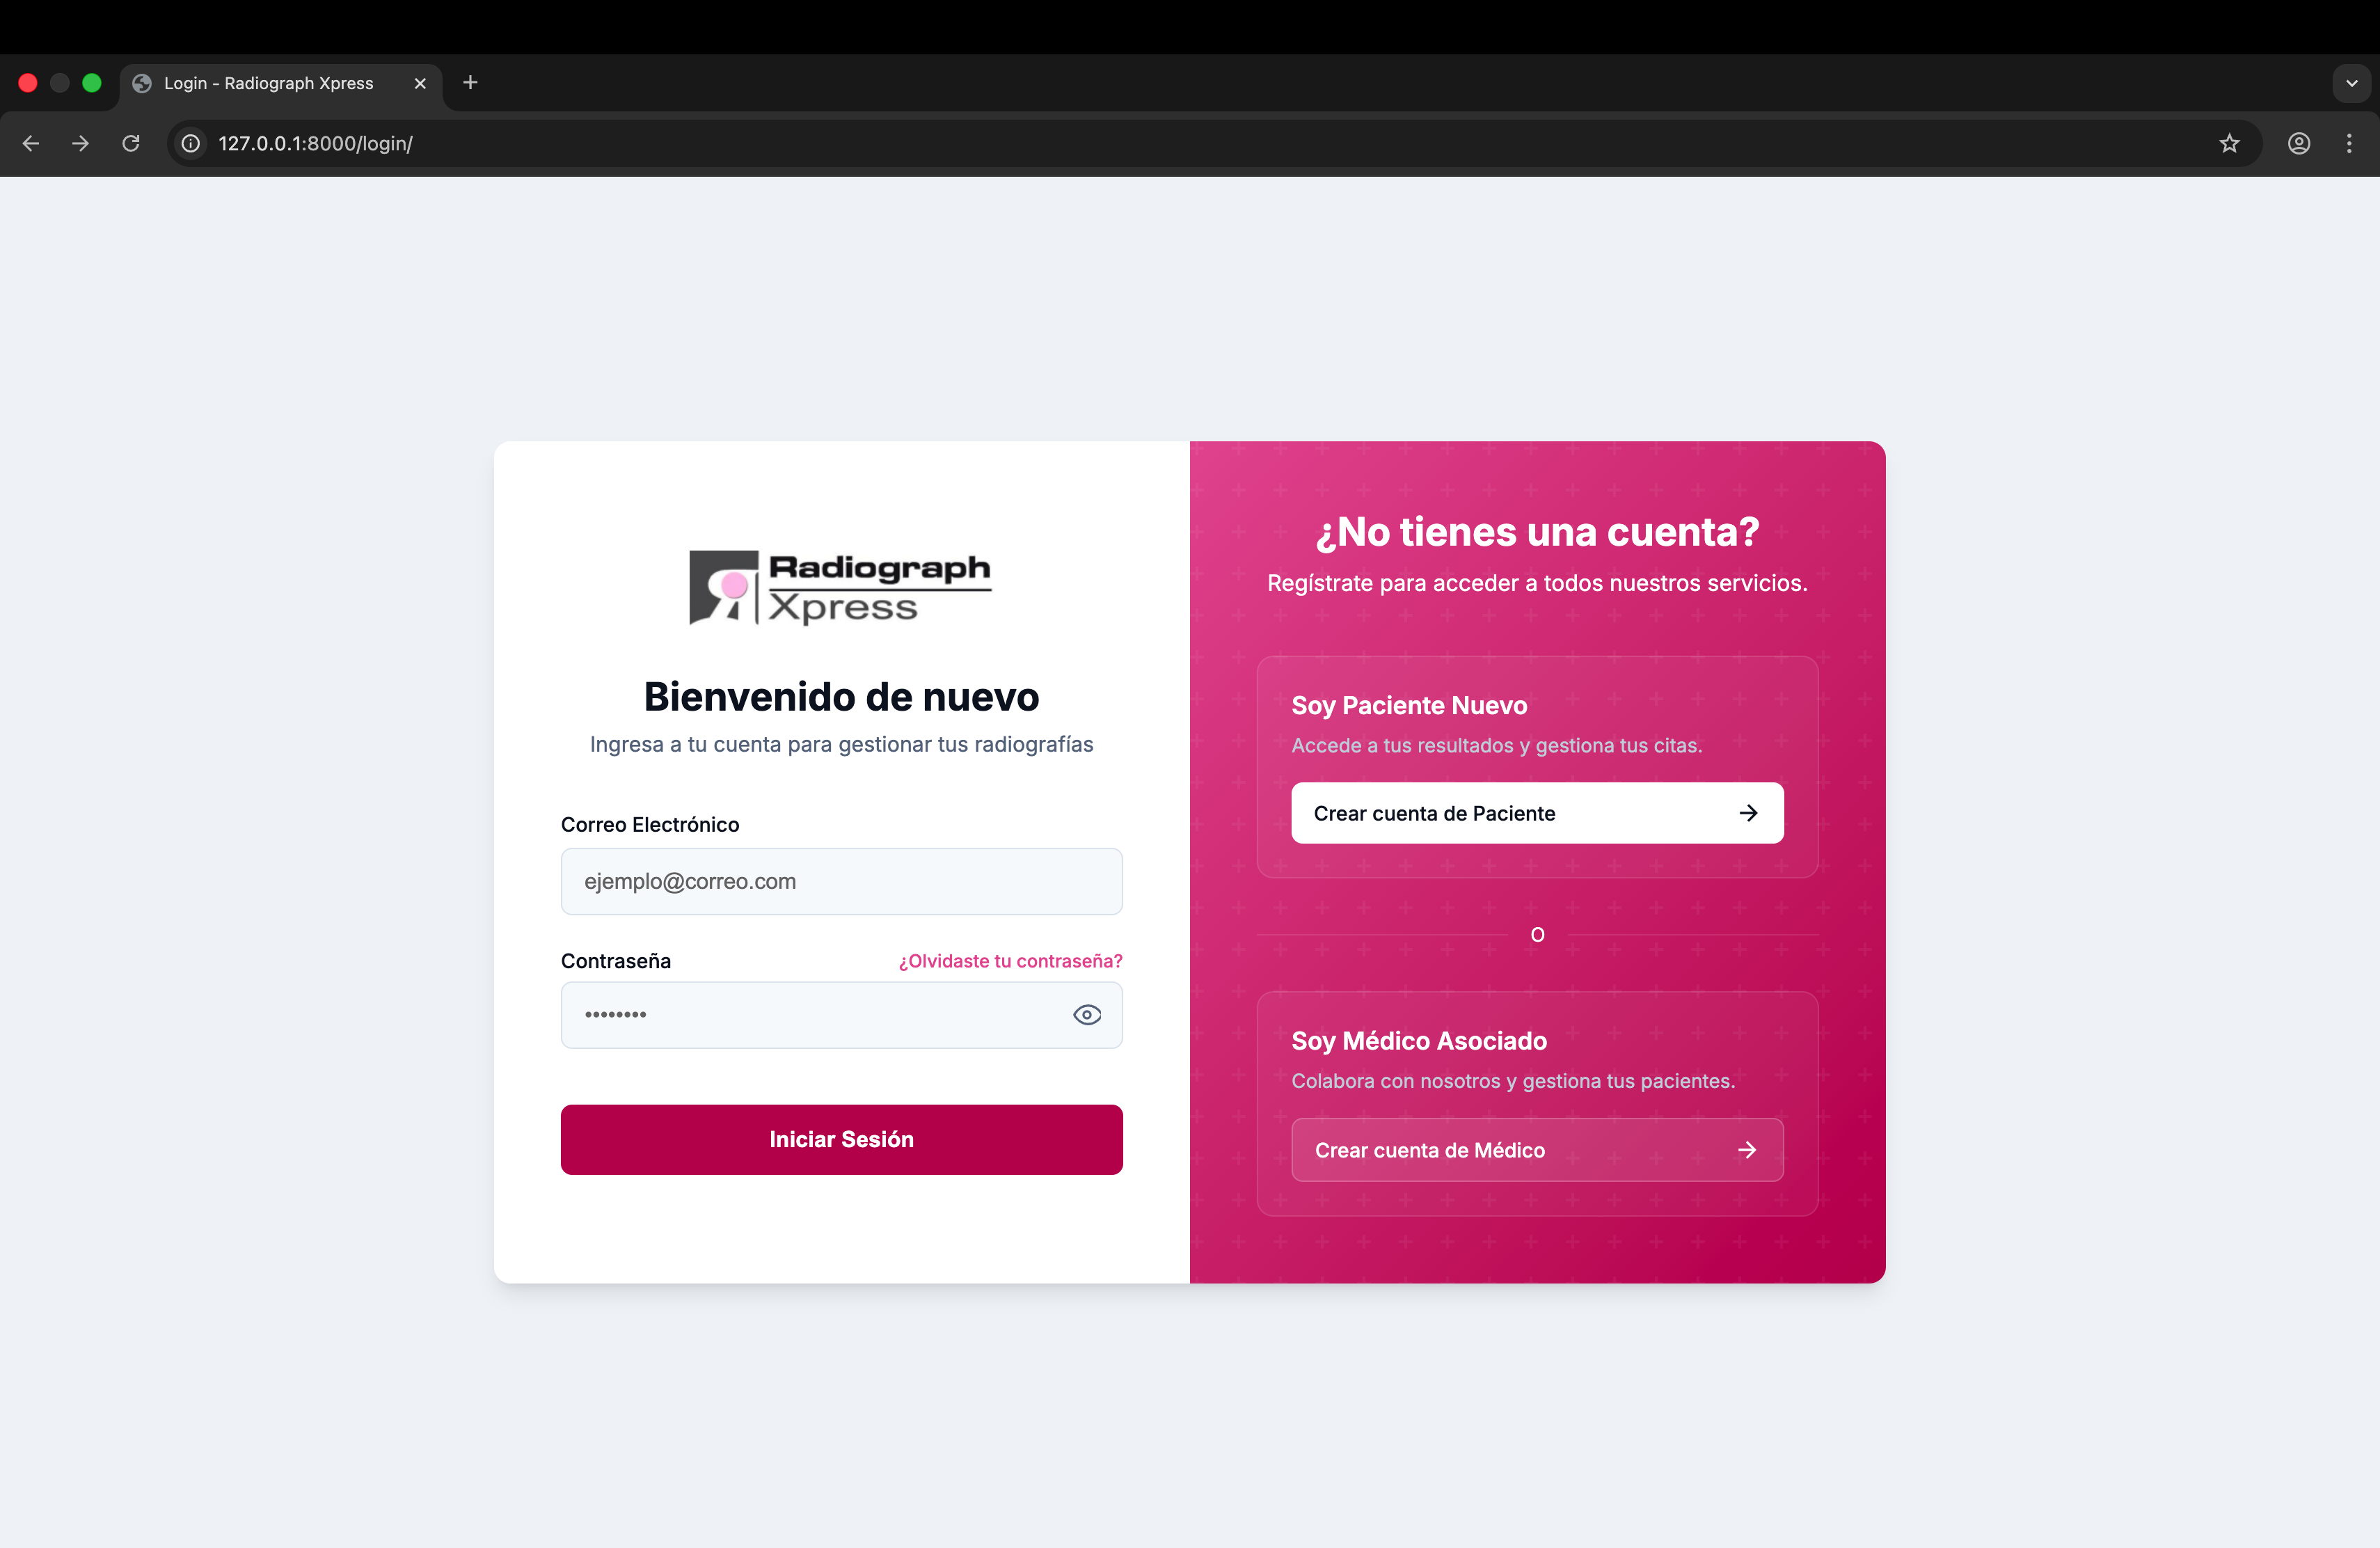
\includegraphics[width=0.7\textwidth]{screenshots/login.png}
        \caption{Pantalla de inicio de sesión genérica.}
    \end{figure}
\end{enumerate}
